%----------------------------------------------------------------------------------------
%	CLASS, PACKAGES AND OTHER DOCUMENT CONFIGURATIONS
%----------------------------------------------------------------------------------------
\documentclass[
	a4paper, % Paper size, use either a4paper or letterpaper
	12pt, % Default font size, the template is designed to look good at 12pt so it's best not to change this
	%unnumberedsections, % Uncomment for no section numbering
]{CSSullivanBusinessReport}
\usepackage{tikz}
\usetikzlibrary{arrows.meta,
                chains,
                positioning}
\addbibresource{references.bib} % BibLaTeX bibliography file
\usepackage{float} % for [H] option

%----------------------------------------------------------------------------------------
%	REPORT INFORMATION
%----------------------------------------------------------------------------------------

\reporttitle{CARE Lab Social Engineering Competition} % The report title to appear on the title page and page headers, do not create manual new lines here as this will carry over to page headers

\reportsubtitle{Day One Deliverables} % Report subtitle, include new lines if needed

\reportauthors{\textbf{Authors:}\\\smallskip Liam Geyer (lfg5289@psu.edu)\\\smallskip Jenna Fox (jef5600@psu.edu)\\\smallskip Brendan McShane (bbm5360@psu.edu)\\\smallskip Jonathan Skeete (jxs7245@psu.edu)} % Report authors/group/department, include new lines if needed

\reportdate{April 19, 2024} % Report date, include new lines for additional information if needed

\rightheadercontent{\includegraphics[height=1.5cm]{assets/branding/ccso-shield.png}} % Header logo

%----------------------------------------------------------------------------------------

\begin{document}

%----------------------------------------------------------------------------------------
%	TEMPLATE PAGES
%----------------------------------------------------------------------------------------

\input{template/title-page.tex}
\begin{twothirdswidth} % Content in this environment to be at two-thirds of the whole page width
	\tableofcontents % Output the table of contents, automatically generated from the section commands used in the document
\end{twothirdswidth}

\newpage

%----------------------------------------------------------------------------------------
%	SECTIONS
%----------------------------------------------------------------------------------------

\section{Executive Summary} % Top level section
\begin{fullwidth}
The CARE Lab fraud fighters team was solicited to assist a young student, Sam, with determining the legitimacy of a job opportunity she recently received. During the first day of the engagement the team met with Sam's friends to gather background information on both the employment opportunity and Sam.\\\medskip

Sam initially posted her resume on an online job seeking site, after which she was quickly contacted by Kellie McDaniel. McDaniel claimed to be from HealthComp, a healthcare solutions company. Sam received an offer to interview for six different positions with David W. Bondeson who was identified as the "Interview Manager". The positions were offered as either full or part time, and fully remote.\\\medskip

The team built a comprehensive profile of the prospective employer, assembled a timeline of events, identified a number of potential red flags, and created a plan to assist Sam throughout the rest of the job seeking process. Notably, the team identified a number of red flags, and a Better Business Bureau scam report consistent with the profile of Sam's prospective employer. With this in mind, the team recommends that should Sam choose to move forward she do so hesitantly, and should consult with the fraud fighting team before disclosing any sensitive information.
\end{fullwidth}
\section{Employer/Scammer Profile} % Top level section
\begin{fullwidth}

\subsection{Employer Profile}
HealthComp is a third-party administrator for healthcare solutions founded in 1994 which helps employers make informed financial decisions regarding self-funded health plans for employees. HealthComp and Virgin Pulse, another healthcare solutions company, merged in November of 2023 in a \$3 billion deal to create a company that uses technology and AI to create health plan designs that improve member health and lower costs \autocite{VirginPulse:2023}. Beginning February of 2024 the merger between Virgin Pulse and HealthComp started its transition to the Personify Health name and brand \autocite{PersonifyHealth:2024}.\\\medskip

HealthComp utilizes an \href{https://careers-virginpulse.icims.com/jobs/intro}{online careers portal} under the banner of Personify Health for its job postings and applications. All of their currently posted remote job listings are full time, and provide a salary range along with detailed descriptions of needed qualifications and duties \autocite{VirginPulse:2024}. The team found no indication that HealthComp commonly solicits interviews without an application.

\subsection{Scammer Profile}
As it pertains to Sam's employment, all emails received only reference HealthComp with no mention of the new brand name, Personify Health. Additionally, the email provided to contact, Mr. David W. Bondeson, is directed towards the email domain @healthcomp.live; however, all contact within the company comes from the @healthcomp.com domain, as seen through the real David W. Bondeson's Linkedin page. \\\medskip

\begin{figure*} % Use the figure* environment for full width figures
        \label{sec:Fig1}
        \centering
	\includegraphics[width=.75\linewidth]{assets/bondeson-email.png}
        \captionsetup{justification=centering}
	\caption{David W. Bondeson's LinkedIn contact information which utilizes the healthcomp.com domain as opposed to the provided healthcomp.live}
\end{figure*}

The message from McDaniel promises flexibility that is not found within the Personify Health job listings. It is also worth noting that the positions referenced in the email: Customer Service Representative, Executive Assistant, Human Resource Assistant, Project Manager, Administrative Assistant, Data Entry, and Content Writer, do not appear on either LinkedIn or the internal job board as well for Personify Health.
\end{fullwidth}
\section{Timeline of Events} % Top level section

\begin{fullwidth}
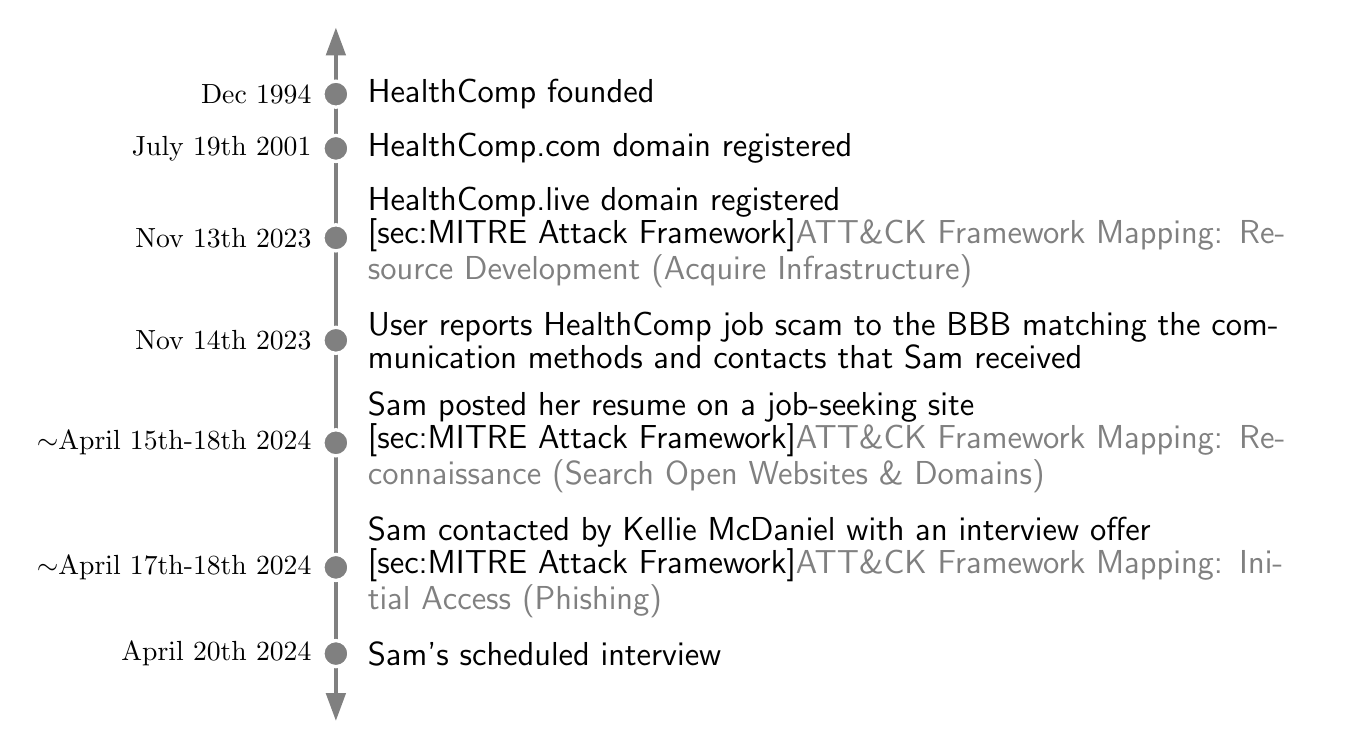
\begin{tikzpicture}[
node distance = 1mm and 3mm,
  start chain = A going below,
   dot/.style = {circle, draw=white, very thick, fill=gray,
                 minimum size=3mm},
   box/.style = {rectangle, text width=120mm,
                 inner xsep=4mm, inner ysep=1mm,
                 font=\sffamily\large\linespread{0.84}\selectfont,
                 on chain},
                        ]
    \begin{scope}[every node/.append style={box}]
    \node { HealthComp founded} ;
    \node { HealthComp.com domain registered} ;
    \node { HealthComp.live domain registered\\
    \hyperref[sec:MITRE Attack Framework]{\textcolor{gray}{ATT\&CK Framework Mapping: Resource Development (Acquire Infrastructure)}}} ;
    \node { User reports HealthComp job scam to the BBB matching the communication methods and contacts that Sam received} ;
    \node { Sam posted her resume on a job-seeking site\\
    \hyperref[sec:MITRE Attack Framework]{\textcolor{gray}{ATT\&CK Framework Mapping: Reconnaissance (Search Open Websites \& Domains)}}} ;
    \node { Sam contacted by Kellie McDaniel with an interview offer\\
    \hyperref[sec:MITRE Attack Framework]{\textcolor{gray}{ATT\&CK Framework Mapping: Initial Access (Phishing)}}} ;
    \node { Sam's scheduled interview} ;
    \end{scope}
\draw[very thick, gray, {Triangle[length=10pt)]}-{Triangle[length=10pt]}, % arrow size  
      shorten <=-5.5mm, shorten >=-6mm] % length of arrows
    (A-1.north west) -- (A-7.south west); % number of nodes in timeline
\foreach \i [ count=\j] in {Dec 1994, July 19th 2001, Nov 13th 2023, Nov 14th 2023, $\sim$April 15th-18th 2024, $\sim$April 17th-18th 2024, April 20th 2024}
    \node[dot,label=left:\i] at (A-\j.west) {};
    \end{tikzpicture}
\subsection{Persuasive Techniques}

\begin{enumerate}
    \item \textbf{Recognizance of Achievements}
            \\\medskip
                The email received by Sam begins with HR stating they found her background and qualifications impressive. Beginning with flattery may be an attempt to lower the guard of the recipient, and is usually followed by promises that seem too good to be true.
    \item \textbf{Too Good to be True}
        \\\medskip
                The advertised pay rate is generalized at \$38.11/hr for all six roles which is uncommon since each role would require a different skill set and therefore the salary for each position should be different. The generalization of such a high pay rate is likely a lure so applicants are inclined to follow up with the job offer.
        \\\medskip
                The email sent to Sam offers a work from home opportunity as well as a part-time, flexible schedule; However, all remote positions listed on Personify Health's LinkedIn and internal job board are for full-time employees.
    \item \textbf{Authority}
        \\\medskip
                Sam's point of contact for the interview is Mr. David W. Bondeson, and although not stated in the email, a google search shows that he's the Director of Stop Loss Sales at Personify Health. Scheduling an interview with an executive at such a high level may make potential employees feel special and reassured about the legitimacy of the opportunity.
    \item \textbf{Masquerade}
        \\\medskip
                Posing as a legitimate company builds trust between the employer and interviewee. If the job offer was sent from a company with little to no online presence, potential victims would be more wary in continuing contact with Human Resources.
\end{enumerate}

\subsection{MITRE ATT\&CK Framework Mappings}

\begin{enumerate}
    \item \textbf{Resource Development: Acquire Infrastructure T1583}
            \\\medskip On Nov 13, 2023 the healthcomp.live domain is registered for use in later scams and phishing campaigns. This maps closely with the first \hyperref[sec:BBB Scam Report]{reported HealthComp scam} which was reported the next day.
    \item \textbf{Reconnaissance: Search Open Websites \& Domains T1593}
            \\\medskip Sam posted her resume to a public job-seeking site somewhere between April 15th-18th 2024. She was contacted shortly offer with the interview offer from Kellie McDaniel. The scam perpetrators likely utilized open source intelligence techniques to find her job site posting and identify her as a target for their scam.
    \item \textbf{Initial Access: Phishing T1566}
            \\\medskip On either April 17 or 18, 2024 Sam was sent what the team believes to be a phishing email, specifically a job scam. This serves as the point of initial access for future exploitation of the target.
\end{enumerate}

\end{fullwidth}
\section{Red Flags} % Top level section
\begin{fullwidth}
During the course of the initial interview with Sam's friends, the fraud fighting team identified a number of potential red flags with the HealthComp job opportunity.

\subsection{Email Red Flags}
The email that Sam received contains multiple red flags that indicate that it may be a phishing email. These include:
\begin{itemize}
	\item Numerous grammatical errors \hyperref[sec:NIST Phish Scale]{(NIST Phish Scale Cue Type: Error)}
        \begin{itemize}
            \item Several misspelled words \hyperref[sec:Fig2]{(See Figure 2)}
            \item Several missed commas \hyperref[sec:Fig3]{(See Figure 3)}
            \item Several run on sentences \hyperref[sec:Fig4]{(See Figure 4)}
            \item Discrepancies with how David Bondeson is titled
            \hyperref[sec:Fig5]{(See Figure 5)}
        \end{itemize}
    \item Email address referenced in email is healthcomp.live \hyperref[sec:NIST Phish Scale]{(NIST Phish Scale Cue Type: Technical Indicators)}
        \begin{itemize}
            \item healthcomp.live is not utilized by HealthComp, the company uses healthcomp.com for email communication
            \item The healthcomp.live domain was recently registered
        \end{itemize}
    \item Sender Kellie McDaniel is not listed as a HealthComp employee \hyperref[sec:NIST Phish Scale]{(NIST Phish Scale Cue Type: Technical Indicators)}
	\item Email signed by HealthComp instead of the sender or an HR Representative \hyperref[sec:NIST Phish Scale]{(NIST Phish Scale Cue Type: Language and Content)}
	\item Email is generically addressed to "Candidate" as opposed to Sam \hyperref[sec:NIST Phish Scale]{(NIST Phish Scale Cue Type: Language and Content)}
    \item Utilizes a "verification code" as opposed to applicant name
\end{itemize}

\subsubsection{Grammatical Errors}

\begin{figure*}[H] % Use the figure* environment for full width figures
    \label{sec:Fig2}
    \centering
    \includegraphics[width=.75\linewidth]{assets/misspelling.png}
    \captionsetup{justification=centering}
    \caption{Misspelling of "fitment". It should just say "fit".}
\end{figure*}

\begin{figure*}[H] % Use the figure* environment for full width figures
    \label{sec:Fig3}
    \centering
    \includegraphics[width=.75\linewidth]{assets/missedCommas.png}
    \captionsetup{justification=centering}
    \caption{There should be a comma following "\$27/hr" and before "but".}
\end{figure*}

\begin{figure*}[H] % Use the figure* environment for full width figures
    \label{sec:Fig4}
    \centering
    \includegraphics[width=.75\linewidth]{assets/runon.png}
    \captionsetup{justification=centering}
    \caption{This is a run-on sentence that should be broken up into two or three separate sentences.}
\end{figure*}

\begin{figure*}[H] % Use the figure* environment for full width figures
    \label{sec:Fig5}
    \centering
    \includegraphics[width=.75\linewidth]{assets/titleerror.png}
    \captionsetup{justification=centering}
    \caption{Discrepancy between "Mr.David W. Bondeson" compared to "Mr David W. Bondeson".}
\end{figure*}

\subsection{Job Red Flags}
The job posting includes various red flags. These include:
\begin{itemize}
	\item Job interview is for 6 different positions
        \begin{itemize}
            \item All jobs have the same pay rate despite different duties and skill levels \hyperref[sec:Fig6]{(See Figure 6)}
            \item All jobs are fully remote and create your own schedule \hyperref[sec:Fig7]{(See Figure 7)}
            \item None of the jobs are listed on the HealthComp careers website \hyperref[sec:Fig8]{(See Figure 8)}
        \end{itemize}
    \item Interview is scheduled through a text based chat instead of phone, video, or in person.
    \item On LinkedIn, David is listed as "Director of Stop Loss Sales", a director is not likely to conduct an interview for an entry level position \hyperref[sec:Fig1]{(See Figure 1)}
\end{itemize}

\subsubsection{Job Posting Evidence}

\begin{figure*}[H] % Use the figure* environment for full width figures
    \label{sec:Fig6}
    \centering
    \includegraphics[width=.75\linewidth]{assets/positions.png}
    \captionsetup{justification=centering}
    \caption{The email specifies these six job positions as available.}
\end{figure*}

\begin{figure*}[H] % Use the figure* environment for full width figures
    \label{sec:Fig7}
    \centering
    \includegraphics[width=.75\linewidth]{assets/remoteSched.png}
    \captionsetup{justification=centering}
    \caption{The email specifies all jobs are work-from-home and have custom schedules.}
\end{figure*}

\begin{figure*}[H] % Use the figure* environment for full width figures
    \label{sec:Fig8}
    \centering
    \includegraphics[width=1\linewidth]{assets/realJobPosting.png}
    \captionsetup{justification=centering}
    \caption{The job listings for HealthComp do not have the offered position of content writer available}
\end{figure*}

\subsection{BBB Scam Report}
\label{sec:BBB Scam Report}

The team found a report submitted to the Better Business Bureau which fits the exact description of Sam's interactions with the prospective employer.

\begin{quote}
	\textbf{\LARGE ``}I was sent an email about a potential job offer for HealthComp I then got instructions to conduct an interview on Microsoft Team then they so called hired me and had me fill out paper work including a W4 form that had my ssn number then after that I told them I had finished filling out the paper work and then they started asking if I was going to be using a credit card to accept my payments and I said no then they said I need one so they can process faster then that's when I realized it was a scam\textbf{''}
	
	\hfill--- BBB Scam ID \#772647 \autocite{BBB:2023}
\end{quote}

The BBB Scam Report lists the same davidbondeson@healthcomp.live email address referenced in Sam's interview offer. With this in mind, it's extremely likely that Sam's job opportunity is not legitimate.
\end{fullwidth}
\section{Gameplan} % Top level section
\begin{fullwidth}
The team's goal is to help guide Sam through this potential job scam using the evidence collected from OSINT and today's preliminary interview. During the rest of Sam's hiring process the team intends to guide her through the interview, and prevent Sam from falling victim to an employment scam.\\\medskip

During the interview the team will continue to evaluate the interaction to see if it is consistent with the characteristics of a job scam. Specifically, it's imperative to see if the interview and hiring process follow the same formula outlined in the \hyperref[sec:BBB Scam Report]{BBB Scam Report}. If this is the case, the team will advise Sam not to disclose any sensitive or personal information in order to avoid both financial loss and identity theft.\\\medskip

Additionally, the team plans to educate Sam on the different types of common job scams to better equip her for the rest of her job search. The team will develop a guide on identifying scams and fraud, and checklists for victims of scams that Sam can utilize in the future. It's encouraged that Sam take a proactive approach to preventing these scams in the future, by scrutinizing suspicious opportunities, and avoiding posting publicly.
\end{fullwidth}

%----------------------------------------------------------------------------------------
%	 REFERENCES/BIBLIOGRAPHY
%----------------------------------------------------------------------------------------

\newpage

\addcontentsline{toc}{section}{References} % Add the bibliography to the table of contents

\begin{twothirdswidth} % Content in this environment to be at two-thirds of the whole page width
	\printbibliography[title=References] % Output the bibliography with a custom section title
\end{twothirdswidth}

%----------------------------------------------------------------------------------------
%	APPENDICES
%----------------------------------------------------------------------------------------

\newpage

\section*{Appendices}

\begin{appendices}

\begin{fullwidth}
\section{NIST Phish Scale}
\label{sec:NIST Phish Scale}

The NIST Phish scale was developed by NIST to identify phishing attacks and evaluate the effectiveness of training to combat these attacks. The scale evaluates the complexity and quality of a phishing attack so that organizations can better train their employees and/or clients to identify these attacks \autocite{Dawkins:2023}.

NIST considers the following criteria in an email when assessing a phishing attack:
\begin{enumerate}
    \item \textbf{Error}: Spelling errors, grammatical errors, and inconsistencies.
    \item \textbf{Technical Indicator}: Attachment types, sender email, sender information, hyperlinks, and domains used.
    \item \textbf{Visual Presentation Indicator}: Professionalism of the email, company logos, and other visual elements that would be expected in a cooperate email. 
    \item \textbf{Language and Content}: Threats presented by the email writer, urgency, lack of details, and/or irrelevant details.
    \item \textbf{Common Tactic}: Such as too good to be true offers, special treatment, and/or posing as a friend/colleague/employer.
\end{enumerate}

NIST also considers the premise alignment of the communications to indicate how difficult it is for a victim to detect. Premise alignment is a measure of how closely an email matches the work roles or responsibilities of an email’s recipient or organization. The stronger an email’s premise alignment, the more difficult it is to detect as a phish. Inversely, the weaker an email’s premise alignment, the easier it is to detect as a phish \autocite{Dawkins:2023}.

The following premise alignment attributes are assessed on the NIST phish scale:
\begin{enumerate}
    \item \textbf{Mimics a Workplace Process or Practice}: The closer a phishing email mimics how an organization acts, the more likely the target is to fall for the phishing attack.
    \item \textbf{Has Workplace Relevance}: If the attack takes the target's job position and workplace access into account, they target is more likely to find the email legitimate.
    \item \textbf{Aligns With Situations or Events}: Should the message be timely to events occurring in the target's life or organization, the target is more likely to believe that the message is legitimate.
    \item \textbf{Engenders Concern Over Consequences}: If the email is threatening the target to take action or face consequences, the target is more likely to perform the requested actions in order to avoid the consequences, even if the consequences do not exist.
    \item \textbf{Training/Experience of Recipient With Phishing Emails}: When the target is trained in identifying phishing attacks, or has previously been a victim to phishing attacks, they are more likely to identify the attack and stop it.
\end{enumerate}

\end{fullwidth}
\begin{fullwidth}
\section{MITRE ATT\&CK Framework}
\label{sec:MITRE Attack Framework}
The MITRE ATT\&CK Framework catalogs cybercriminal's tactics, techniques and procedures in each phase of their attack. This allows defenders to identify such attack methods and ensure that their defenses are capable of stopping such attacks \autocite{IBM}.

The attack framework is ordered chronologically, with 1 being the first phase of the attack and 14 being the last phase of the attack. Each phase of the MITRE ATT\&CK Framework is as follows:

\begin{enumerate}
    \item \textbf{Reconnaissance}: gather information about the target to plan for an attack.
    \item \textbf{Resource Development}: build and acquire resources to carry out the attack. This can include domains, web sites, and email servers.
    \item \textbf{Initial Access}: Exploit the target to get initial access to their environment.
    \item \textbf{Execution}: Run malware or malicious code on the exploited system.
    \item \textbf{Persistence}: Setup access to the system that will withstand reboots or system reconfiguration.
    \item \textbf{Privilege Escalation}: Gain access to accounts with higher privileges, such as an administrator.
    \item \textbf{Defense Evasion}: Avoid detection, such as anti-virus or intrusion detection systems.
    \item \textbf{Credential Access}: Gather usernames, passwords, and other credentials to expand access.
    \item \textbf{Discovery}: Explore and research the target's system to find systems that can be accessed or controlled to support an attack.
    \item \textbf{Lateral Movement}: Gain access to other resources in the environment.
    \item \textbf{Collection}: Gather target's data in the environment related to the goal.
    \item \textbf{Command and Control}: Establish covert/undetectable communications from the target's systems to the attacker that enable control over the target's system.
    \item \textbf{Exfiltration}: Steal data from the target's system.
    \item \textbf{Impact}: Interrupt the business' function and data.
\end{enumerate}
\end{fullwidth}

\end{appendices}

%----------------------------------------------------------------------------------------

\end{document}
